\chapter{Incorporation of Dynamic Tubes for Constraint Satisfaction and Extension to Multiple Agents}
\label{sec:dynamic-tube}
Following the determination of the docking point of the chaser, the chaser plans a trajectory from the current position to the calculated goal position on the target.
As a result of SMID-based adaptive control, the chaser has significantly improved estimates of uncertain parameters (eccentricity and drag constant) by the completion of rendezvous and it is capable of planning a trajectory from a start position to a docking point on the target.
However, while the docking point is on the surface of the target, the target also behaves as an obstacle in the trajectory planning problem of the chaser.
The resulting high degree of proximity from physical contact required for docking increases the likelihood of a chaser-target collision.
While the time-varying docking constraint (Section \ref{sec:time-varying-collision-constraints}) prevents the nominal state from such a collision, the inaccuracy in estimated parameters may lead to a violation of this constraint.

In order to avoid such constraint violations, we use dynamic robust control-invariant (RCI) tubes as proposed in \cite{brett2019dynamic} to constrain the possible error in the chaser state, hence using adaptive dynamic tube MPC (ADTMPC) for chaser trajectory planning.
As a result, the general nominal trajectory planning problem can be formulated as the following optimization problem:
\begin{align}
    \min_{\hat{\boldsymbol{u}}}\ J(\hat{\boldsymbol{r}},\hat{\boldsymbol{u}})&=h(\hat{\boldsymbol{r}}(\theta_f))+\int_{\theta_0}^{\theta_f} \left((\hat{\boldsymbol{r}}-\boldsymbol{r}_f)^TQ(\hat{\boldsymbol{r}}-\boldsymbol{r}_f)+\hat{\boldsymbol{u}}^TR\hat{\boldsymbol{u}}\right)d\theta\label{eqn:dynamic-tubes-equation}
\end{align}
\addtocounter{equation}{-1}
\vspace{-4ex}
\begin{subequations}
\begin{align}
    \textrm{s.t. } & \hat{\boldsymbol{r}}'=A(\theta)\hat{\boldsymbol{r}}+B(\theta)\hat{\boldsymbol{u}}+\hat{\boldsymbol{d}}(\theta), \ \ \hat{\boldsymbol{u}}\in\hat{\mathcal{U}},\\
    & \hat{\boldsymbol{r}}(\theta_0)=\boldsymbol{r}(\theta_0)=\boldsymbol{r}_0,\quad\hat{\boldsymbol{r}}\in\hat{{\mathcal{C}}},\\
    & \boldsymbol{\phi}'=-\hat{\boldsymbol{\alpha}}\boldsymbol{\phi}+\boldsymbol{\Delta}(\hat{\boldsymbol{r}})+\boldsymbol{D}+\boldsymbol{\eta},\ \ \boldsymbol{\phi}(\theta_0)=\boldsymbol{\phi}_0,\\
    & \boldsymbol{\Omega}'=A_\lambda\boldsymbol{\Omega}+B_\lambda\boldsymbol{\phi},\quad\boldsymbol{\Omega}(\theta_0)=|\Tilde{\boldsymbol{r}}_0|,
\end{align}
\end{subequations}
where $A_\lambda=\text{diag}(\boldsymbol{\lambda})=\text{diag}([\lambda_1,~\lambda_2,~\lambda_3])$, $B_\lambda=I_{3}$, and $h(\cdot)$ and $\hat{{\mathcal{C}}}$ are determined based on the operation, e.g., rendezvous or docking.
Here, $\phi(\theta)$ represents the boundary layer of the tube and $\Omega(\theta)$ represents the tube geometry.
Also, $\hat{{\mathcal{C}}}$ refers to the tightened set of constraints discussed in detail in Sections \ref{sec:bound-shrinking} and \ref{sec:non-convex_const_expansion}.
\begin{figure}[htb]
    \centering
    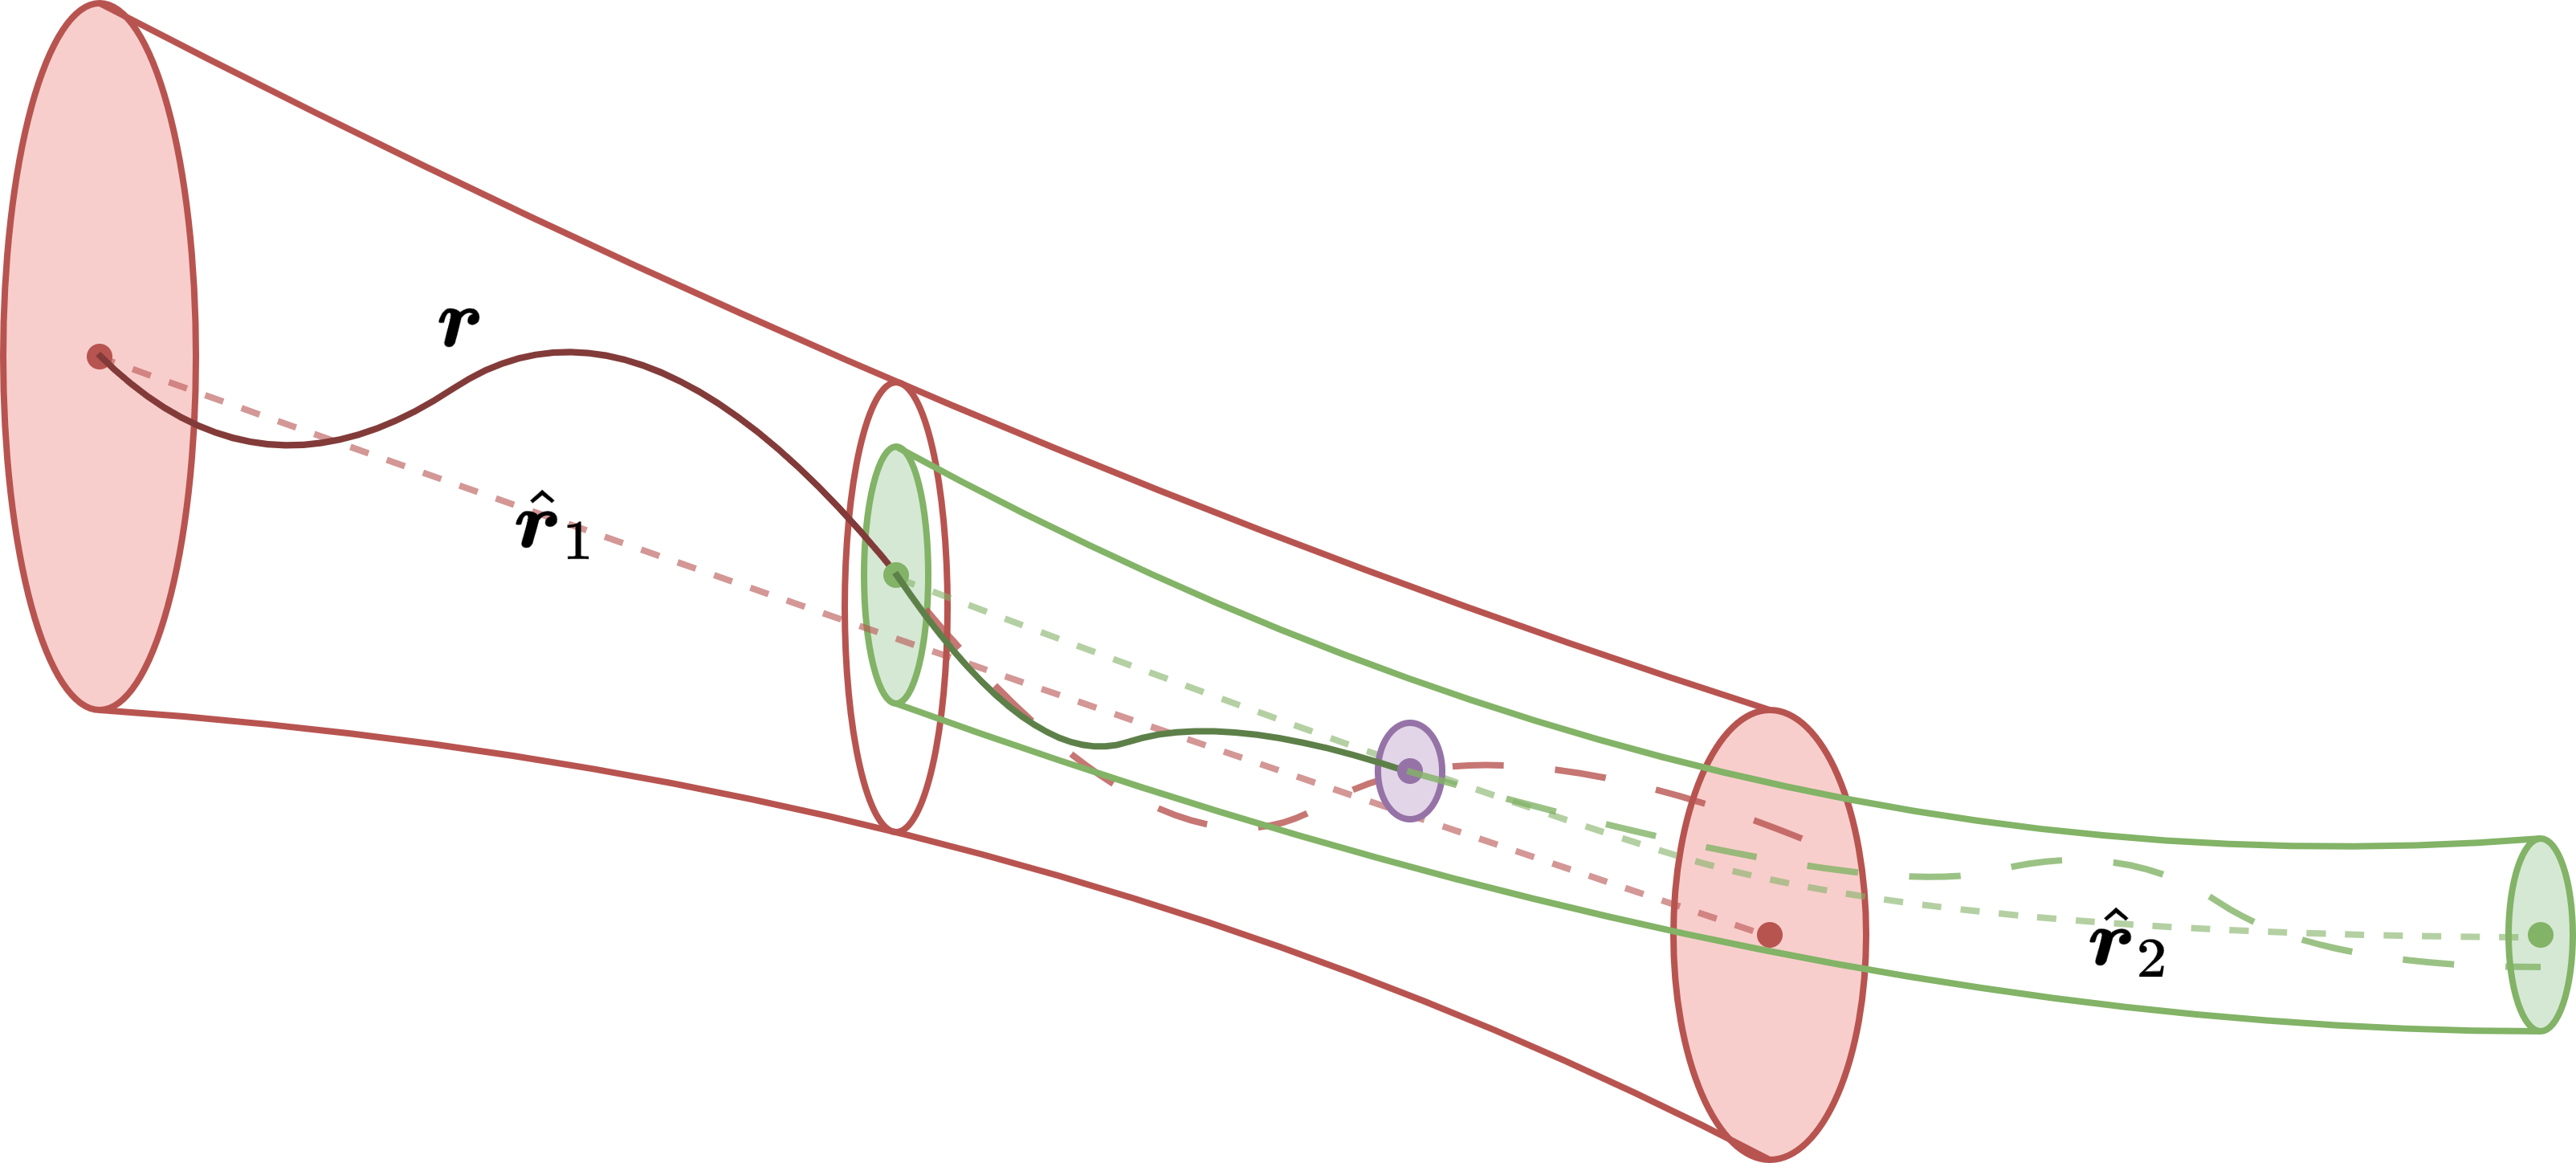
\includegraphics[width = 0.96\linewidth]{assets/adtmpc.png}
    \caption{Adaptive Tube Model Predictive Control. The tubes represent the permissible region for the actual trajectory of the chaser. The dotted lines represent the nominal states and the dashed lines represent the actual states. Due to the receding horizon nature of the problem, the spacecraft plans a new trajectory before the final state is reached.}
    \label{fig:adtmpc}
\end{figure}
\section{Ancillary Controller and the Actual Control Input}
The boundary-layer sliding mode controller (BLSC) that supports the robust tube mechanism is introduced as an ancillary controller to the nominal input that is obtained from the trajectory planning problem.
Hence, the actual control input $\boldsymbol{u}$ can be written as the sum of the nominal input $\hat{\boldsymbol{u}}$ and this ancillary controller $\Tilde{\boldsymbol{u}}$:
\begin{alignat}{2}
    \boldsymbol{u}&=\hat{\boldsymbol{u}}+\Tilde{\boldsymbol{u}},\\
    \Tilde{\boldsymbol{u}}&=B(\boldsymbol{r})^{-1}\left(A^V\Tilde{\boldsymbol{r}}-A_\lambda\Tilde{\boldsymbol{v}}-\text{sat}\left(\frac{\boldsymbol{s}}{\boldsymbol{\phi}}\right)[K(\boldsymbol{r})]\right),
\end{alignat}
where the sliding variable $\boldsymbol{s}$ is defined as:
\begin{alignat}{2}
    \boldsymbol{s}=\Tilde{v}+A_\lambda\Tilde{p},
\end{alignat}    
and $[K(\boldsymbol{r})]=\text{diag}(K(\boldsymbol{r}))$ can be calculated as:
\begin{subequations}
\begin{alignat}{2}
    \boldsymbol{\phi}'&=-\boldsymbol{\alpha}\boldsymbol{\phi}+\boldsymbol{\Delta}(\boldsymbol{r})+\boldsymbol{D}+\boldsymbol{\eta},\\
    K(\boldsymbol{r})&=\boldsymbol{\Delta}(\boldsymbol{r})+\boldsymbol{D}+\boldsymbol{\eta}-\phi'\\
    &=(\boldsymbol{\Delta}(\boldsymbol{r})-\boldsymbol{\Delta}(\hat{\boldsymbol{r}}))+\boldsymbol{\alpha}\boldsymbol{\phi}\\
    &=\boldsymbol{\Delta}(\Tilde{\boldsymbol{r}})+\boldsymbol{\alpha}\boldsymbol{\phi}.\label{eqn:K(r)}
\end{alignat}
\end{subequations}
Here, $\boldsymbol{\Delta}(\boldsymbol{r})$ is the maximum bound on the dynamics $\boldsymbol{f}=\hat{\boldsymbol{f}}+\Tilde{\boldsymbol{f}}$ where $\hat{\boldsymbol{f}}$ is the nominal dynamics and $\Tilde{\boldsymbol{f}}$ is the bounded model error such that $|\Tilde{\boldsymbol{f}}|\leq\boldsymbol{\Delta}(\boldsymbol{r})$.
Also, $\boldsymbol{D}$ is the maximum bound on the disturbance $\boldsymbol{d}(\theta)$ in the dynamics such that $\boldsymbol{d}(\theta)\leq\boldsymbol{D}$, and $\boldsymbol{\eta}$ is a predefined quantity.
\section{Shrinking of State and Input Bounds}
\label{sec:bound-shrinking}
State and input constraints need to be modified due to the non-zero tracking error $\Tilde{\boldsymbol{r}}(\theta)$.
The state and input bounds defined in Section \ref{sec:state-input-bounds} must be modified to account for the non-zero tracking error and control input error.
We incorporate the tightening equations proposed in \cite{brett2019dynamic} into the optimization problem in Equation \ref{eqn:dynamic-tubes-equation} as a modified set of constraints $\hat{\boldsymbol{r}}\in\hat{{\mathcal{C}}}$ that can be expanded as follows:
\begin{align}
    ||P_{\hat{\boldsymbol{r}}}\hat{\boldsymbol{r}}(\theta)+q_{\hat{\boldsymbol{r}}}||&\leq C_{\hat{\boldsymbol{r}}}-||P_{\hat{\boldsymbol{r}}}\Tilde{\boldsymbol{r}}(\theta)||,\\
    ||P_{\hat{\boldsymbol{u}}}\overline{B}^{-1}\hat{\boldsymbol{u}}(\theta)+q_{\hat{\boldsymbol{u}}}||&\leq C_{\hat{\boldsymbol{u}}}-||P_{\hat{\boldsymbol{u}}}\overline{B}^{-1}\Tilde{\boldsymbol{u}}_{fb}||.
\end{align}
Hence, we may rewrite the state and input bounds as:
\begin{align}
    \hat{\boldsymbol{p}}&\in{\mathcal{P}}:=\{\hat{\boldsymbol{p}}\ |\ |\hat{p}_i|<    \infty\},\quad\text{(no bound)}\\
    \hat{\boldsymbol{v}}&\in{\mathcal{V}}:=\{\hat{\boldsymbol{v}}\ |\ |\hat{v}_i|\leq C_{V}-|\Tilde{v}|\},\\
    \hat{\boldsymbol{u}}&\in{\mathcal{U}}:=\{\hat{\boldsymbol{u}}\ |\ |\hat{u}_i  |\leq C_{U}-|\Tilde{u}_{fb,i}|\},
\end{align}
where $i=1,2,3$ and
\begin{subequations}
\begin{alignat}{2}
    \Tilde{\boldsymbol{u}}_{fb}&=\left|\overline{F}+A_{\lambda}\Tilde{\boldsymbol{r}}\right.&&\left.+\overline{K}\right|,\\
    \overline{F}&=A^V\overline{\boldsymbol{r}},&&\underline{F}=A^V\underline{\boldsymbol{r}},\\
    \overline{K}&=K\left(\overline{\boldsymbol{r}}\right),&&\underline{K}=K\left(\underline{\boldsymbol{r}}\right),\\
    \overline{\boldsymbol{r}}&=\hat{\boldsymbol{r}}+|\Tilde{\boldsymbol{r}}|,&&\underline{\boldsymbol{r}}=\hat{\boldsymbol{r}}-|\Tilde{\boldsymbol{r}}|,
\end{alignat}
\end{subequations}
where $K(\cdot)$ is defined in Equation \ref{eqn:K(r)}.
\section{Expansion of Non-Convex State Constraints}
\label{sec:non-convex_const_expansion}
We realize that, although the inputs are bound in a convex space, the state space is non-convex either due to the radial-limit constraint (Equation \ref{eqn:radial-limit-constraint}) during rendezvous or due to the target-limit constraint (Section \ref{sec:time-varying-collision-constraints}) during docking.
These constraints need to be expanded resembling how the convex bounds are shrunk in Section \ref{sec:bound-shrinking}.
As a result, the radial-limit constraint can now be rewritten as $\hat{\boldsymbol{r}}\in\hat{{\mathcal{C}}}_R$ where:
\begin{alignat}{2}
    \hat{{\mathcal{C}}}_R:=\{\hat{\boldsymbol{r}}\ |\ ||\hat{\boldsymbol{p}}||>\rho_T+||\Tilde{\boldsymbol{p}}||, \rho_T=\min\rho \text{ s.t. } ||\boldsymbol{p}_T||\leq\rho\ \forall\ \boldsymbol{p}_T\in\text{T}\}.
\end{alignat}
Similarly, the chaser-target collision avoidance constraint for docking must be expanded such that the dynamic RCI tube can at most touch the target.
Since distances are invariant to rotations, the expansion of the constraint is not affected by the rotation of the position of the chaser with respect to the target.
As a result, the constraint in Equation \ref{eqn:or-function} can be rewritten as:
\begin{align}
    \hat{{\mathcal{C}}}_D&:=\hat{{\mathcal{C}}}_{D1}\cup\hat{{\mathcal{C}}}_{D2},\label{eqn:expanded-target-limit-constraint}
\end{align}
where
\begin{subequations}
\begin{align}
    \hat{{\mathcal{C}}}_{D1}&:=\{\boldsymbol{r}(\theta)\ |\ f_{D1}\geq0\},\\
    \hat{{\mathcal{C}}}_{D2}&:=\{\boldsymbol{r}(\theta)\ |\ f_{D2}\geq0\}.
\end{align}
\end{subequations}
Here, the constraint functions $f_{D1}$ and $f_{D2}$ are defined as:
\begin{subequations}
\begin{align}
    f_{D1}&=x_{\mathcal{R}}(\theta)^2 + y_{\mathcal{R}}(\theta)^2 - (r_T+||\Tilde{\boldsymbol{p}}||)^2,\\
    f_{D2}&=||z_{\mathcal{R}}(\theta)|| - (l_T+||\Tilde{\boldsymbol{p}}||),
\end{align}
\end{subequations}
We realize that this can be slightly conservative on the edges of the target.
This can be rectified by adding a third constraint while ignoring the existing two constraints at the edge to provide a rounded cylinder constraint.
Similarly, it can be made less conservative by constraining each dimension separately, giving:
\begin{subequations}
\begin{align}
    f_{D1}&=x_{\mathcal{R}}(\theta)^2 + y_{\mathcal{R}}(\theta)^2 - \left(r_T+\left|\left|\begin{bmatrix}
        \Tilde{x}_{\mathcal{R}}&\Tilde{y}_{\mathcal{R}}
    \end{bmatrix}\right|\right|\right)^2,\\
    f_{D2}&=||z_{\mathcal{R}}(\theta)|| - (l_T+||\Tilde{z}_{\mathcal{R}}||),
\end{align}
\end{subequations}
where, for $r_i\in[x,y,z]$,
\begin{align}
    \Tilde{r}_{i, {\mathcal{R}}}=r_{i, {\mathcal{R}}}(\theta)-\hat{r}_{i, {\mathcal{R}}}(\theta).
\end{align}
